\documentclass[math1530-lecture-notes]{subfiles}
\begin{document}

\chapter{Rings: Part II}

\begin{mdframed}
  \textbf{Important}: in this chapter, \textit{ring} means \textit{commutative ring}.
\end{mdframed}

\section{Irreducible Elements and Unique Factorization Domains}

You're likely familiar with the famous theorem that every non-zero integer can be factored uniquely
as a product of primed, the \textbf{Fundamental Theorem of Arithmetic}. We now hope to extend this
concept beyond the integers and into abstract rings, and to explore what unique factorization would
mean for other rings; indeed, some rings have it, and others don't.

From the Fundamental Theorem of Arithmetic, in the ring of integers $\Z$, the primes are the basic
building blocks, where an integer $p\in \Z$ is prime if it does not factor. But that's a lie, since
we can always ``factor'' $p$; for example, we have \[
  p=1\cdot p ~\text{and}~p=(-1)\cdot (-p)
.\] Your first response is, ``that's cheating'', but how exactly is that cheating? If you say to
ignore $\pm 1$, that's correct, but why exactly $\pm 1$, and not anything else?

Let's look at the analogous problem for the polynomial ring $F[x]$, where $F$ is a field. In Chapter
5, we saw the concept of irreducible polynomials, those $f(x)\in F[x]$ that ``do not factor'' in
$F[x]$. But again, that's not exactly true, since for any non-zero constant $c\in F$, we can factor
$f(x)$ into \[
  f(x) = c^{-1}\cdot cf(x)
.\] So when defining non-trivial factorizations in $F[x]$, we need to ignore all non-zero elements
in $F$. 

What do $\pm 1$ in $\Z$ and the non-zero constants in $F[x]$ have in common? \textbf{They're units
in their respective rings}. Recall that 
\begin{definition}[Units]{}
  Let $R$ be a ring. An element $a\in R$ is a \textbf{unit} if it has a multiplicative inverse, i.e.
  if there is an element $b\in R$ satisfying $ab=1$. The set of units of $R$ is denoted $R^*$, which
  is indeed a group with multiplication.
\end{definition}
In general, if $u\in R^*$ is a unit, then we can factor any element $a\in R$ as \[
  a =u^{-1}\cdot u\cdot a
.\] We want to ignore these trivial factorizations; thus, we have our first important definition.
\begin{definition}[Irreducible]{}
  Let $R$ be a ring. A non-zero element $a\in R$ is \textbf{irreducible} if $a$ is not a unit and
  the only way to factor $a=bc$ is if either $b$ or $c$ is a unit.
\end{definition}
As with the unique factorization of integers, it's necessary to carefully define what precisely
uniqueness means. For example, ignoring even the trivial factorizations, the integer $60\in \Z$ has
``multiple different factorizations'': \[
  60=2\cdot 2\cdot 3\cdot 5=2\cdot 3\cdot 5\cdot 2=\ldots
.\] But these factorizations are intrinsically the same; only their orders have changed.

In order to discuss unique factorization in general rings, we thus need to account for potential
ambiguities arising from re-ordering the factors and/or including extra unit factors.
\begin{definition}[Unique Factorization Domain]{}
  Let $R$ be an integral domain, i.e. a commutative ring with no zero divisors. Then $R$ is a
  \textbf{unique factorization domain} (UFD) if:
  \begin{enumerate}
    \item Let $a\in R$ be a non-zero element that is not a unit. Then $a$ can be written in the from
      \[
        a=b_1\cdot b_2\cdot \ldots\cdot b_n
      \] using irreducible elements $b_1,\ldots,b_n\in R$.
    \item Suppose that $b_1,\ldots,b_n\in R,\ c_1,\ldots,c_m\in R$ are irreducible elements of $R$,
      and suppose further that \[
        b_1\cdot b_2\cdot \ldots\cdot b_n=c_1\cdot c_2\cdot \ldots\cdot c_m
      .\] Then $m=n$, and after rearranging $c_1,\ldots,c_n$, there are units $u_1,\ldots,u_n\in
      R^*$ so that \[
        c_1=u_1b_1,\ldots,c_n=u_nb_n
      .\] 
  \end{enumerate}
\end{definition}

Later, we'll show that $\Z$, $\Z[i]$, and $F[x]$ are UFDs. This proof will first show that every
ideal in these rings are principal, then showing that in general, rings with this property are UFDs.

Many rings are not UFDs. For example, the ring \[
  \Z[\sqrt{-3}]=\{a+b\sqrt{-3}\in \C\mid a,b\in \Z \} 
\] is not a UFD (TODO: prove this).

We finish this section with an important class of rings that are UFDs, even though they contain many
non-principal ideals.
\begin{theorem}{}
  Let $F$ be a field. Then the ring $F[x_1,\ldots,x_n]$ of polynomials in $n$ variables with
  coefficients in $F$ is a unique factorization domain. 
\end{theorem}
\begin{proof}[Proof]
  The proof is unfortunately beyond the scope of this chapter. The main key idea is proving that if
  $R$ is a UFD, then $R[x]$ is a UFD; then, we proceed by induction.
\end{proof}

\section{Euclidean Domains and Principal Ideal Domains}

We've seen before the importance of studying ideals of $R$. The simplest ideals are principal
ideals; that is, ideals formed by taking all multiples of a $c\in R$: \[
  cR=(c)=\{rc\mid r\in R\} 
.\] Some rings have the nice property that all ideals are principal.
\begin{definition}[Principal Ideal Domains]{}
  A ring $R$ is a \textbf{principal ideal domain} (PID) if it is an integral domain in which every
  ideal of $R$ is principal.
\end{definition}

We already know two examples of PIDs. The first is the ring of integers $\Z$ [TODO: insert proof].
The second is the ring of polynomials $F[x]$ with coefficients in a field $F$; see Theorem 5.21. In
both cases, the key to proving the PID property is division-with-remainder, as described for $\Z$ in
the prelude and $F[x]$ in Proposition 5.20. This motivates the next definition, which generalizes
the idea of ``division-with-remainder''. The idea is that we want to ``divide'' $a$ by $b$ to get a
quotient $q$ and a remainder $r$, where $r$ is ``smaller'' than $b$. The subtle part here is to
define what exactly it means for an element of a ring to be ``smaller'' than another, and what
properties ``smallness'' should obey.

\begin{definition}[Euclidean Domains]{}
  A ring $R$ is a \textbf{Euclidean domain} if it is an integral domain and if there is a
  \textbf{size function} \[
    \sigma:R\longrightarrow \{ 0,1,2,3,\ldots \}
  \] with the following properties:
  \begin{enumerate}
    \item $\sigma(a)=0$ if and only if $a=0$;
    \item For all $a,b\in R$ with $b\neq 0$, there exist elements $q,r\in R$ that satisfy \[
          a=bq+r~\text{and}~\sigma(r)<\sigma(b)
      .\] 
    \item For all $a,b\in R$, we have $\sigma(ab)=\sigma(a)\sigma(b)$\footnote{Sometimes, only the
      weaker property $\sigma(a)\le \sigma(a)\sigma(b)$ for all non-zero $a,b$ is required.}.
  \end{enumerate}
\end{definition}
We now prove that every Euclidean domain is a principal ideal domain.
\begin{theorem}[]{}
  Every Euclidean domain is a PID.
\end{theorem}
\begin{proof}[Proof]
  Let $R$ be a Euclidean domain with size function $\sigma$, and let $I$ be an ideal of $R$. If
  $I=(0)$, it is clearly principal, so consider $I\neq (0)$. We consider the following set of
  non-negative integers: \[
    \{\sigma(c)\mid c\in I,\ c\neq 0 \} 
  .\] This set is non-empty, since $I\neq (0)$. Therefore this set has a smallest element, say
  $\sigma(b)$. In other words, there is a non-zero element $b\in I$ satisfying \[
    \sigma(b)\le \sigma(c) ~\text{for all}~c\in I
  .\] We claim that $I=(b)$. Let $a\in I$ be any element. Since $R$ is a Euclidean domain, we can
  find elements $q,r\in R$ such that \[
    a=bq+r,\ \sigma(r)<\sigma(b)
  .\] Since $a,b\in I$ and $I$ is an ideal, we have \[
    bq\in I~\text{and hence}~r=a-bq\in I
  .\] Thus $r\in I$ and $\sigma(r)<\sigma(b)$. Since $\sigma(b)\le \sigma(c)$ for any non-zero
  element, we must have that $r=0$. In other words, $a=bq$, so $a\in (b)$. Since we've proved that
  every $a\in I$ is in $(b)$, we have $I\subseteq (b)$. By the definition of an ideal, $(b)\subseteq
  I$, so we have $I=(b)$. Therefore every ideal in a Euclidean domain is principal.
\end{proof}

The ring $\Z$ is a Euclidean domain using the function $\sigma(b)=\left| b \right| $. The formula
$a=bq+r$ just says that dividing $a$ by $b$ gives a quotient $q$ and remainder $r$ with $\left| r
\right| <\left| b \right| $ (see Division Algorithm for integers). Thus $\Z$ is a PID.

Let $F$ be a field. The ring $F[x]$ of polynomials is a Euclidean domain using the size function \[
  \sigma(p(x))=\left\{\begin{array}{lr}2^{\deg{p(x)}} & ~\text{if}~p(x)\neq 0,\\
    0&~\text{if}~p(x)=0\end{array}\right.
\] Indeed, $\sigma$ satisfies the three properties of a size function:
\begin{itemize}
  \item Clearly, $\sigma(p(x))=0$ if and only if $p(x)=0$.
  \item Proposition 5.20 gives us the division algorithm for polynomials; that is, for polynomials
    $f(x),g(x)\in F[x]$, there exist $q(x),r(x)\in F[x]$ satisfying \[
      f(x)=g(x)q(x)+r(x),\ \deg{(r)}<\deg{(g)}
    .\]
  \item The multiplication property is immediate from the fact that the degree of a product of
    polynomials is the sum of their degrees, so \[
      \sigma(p_1p_2)=2^{\deg{p_1}+\deg{p_2}}=2^{\deg{p_1}}\cdot 2^{\deg{p_2}}=\sigma(p_1)\sigma(p_2)
    .\] 
\end{itemize}

Thus $F[x]$ and $\Z$ are PIDs. Another interesting example is the Gaussian integers.
\begin{proposition}{}
  The ring of Gaussian integers $\Z[i]$ is a Euclidean domain using the size function \[
    \sigma(a+bi)=a^2+b^2
  .\]
\end{proposition}
\begin{proof}[Proof]
  The ring $\Z[i]$ is a subring of the field $\C$ of complex numbers, and fields are always integral
  domains; thus $\Z[i]$ is automatically an integral domain. The hard part is proving that $\Z[i]$
  has the Euclidean property using the size function $\sigma$. We'll leave it to you to check that
  \begin{itemize}
    \item $\sigma(\alpha)=0$ if and only if $\alpha=0$;
    \item $\sigma(\alpha\beta)=\sigma(\alpha)\sigma(\beta)$
  \end{itemize}
  We view the field of complex numbers $\C$ as forming the $xy$-plane, with the point $(x,y)$
  corresponding to the complex number $x+yi$. Then the ring $\Z[i]$ consists of the points $(a,b)$
  with integer coordinates, and the size $\sigma(a+bi)$ is the square of the distance from $(0,0)$
  to $(a,b)$.

  We now proceed with a geometric argument. Let $\alpha,\beta\in \Z[i]$ with $\beta\neq 0$. Our task
  is to divide $\alpha$ by $\beta$ to get a quotient $\gamma$ and remainder $\rho$ with
  $\sigma(\rho)<\sigma(\beta)$. The idea is to take the quotient $\alpha / \beta$ and round the
  coefficients to the nearest integer. $\alpha / \beta$ is a complex number, so we plop it into $\C$
  and find its closest element in $\Z[i]$, as illustrated below. The star represents the quotient
  $\alpha / \beta$, while points in $\Z[i]$ are marked with dots. We then picked the closest corner
  to $\alpha / \beta$ and called it $\gamma$.
  \begin{figure}[htpb]
    \centering
    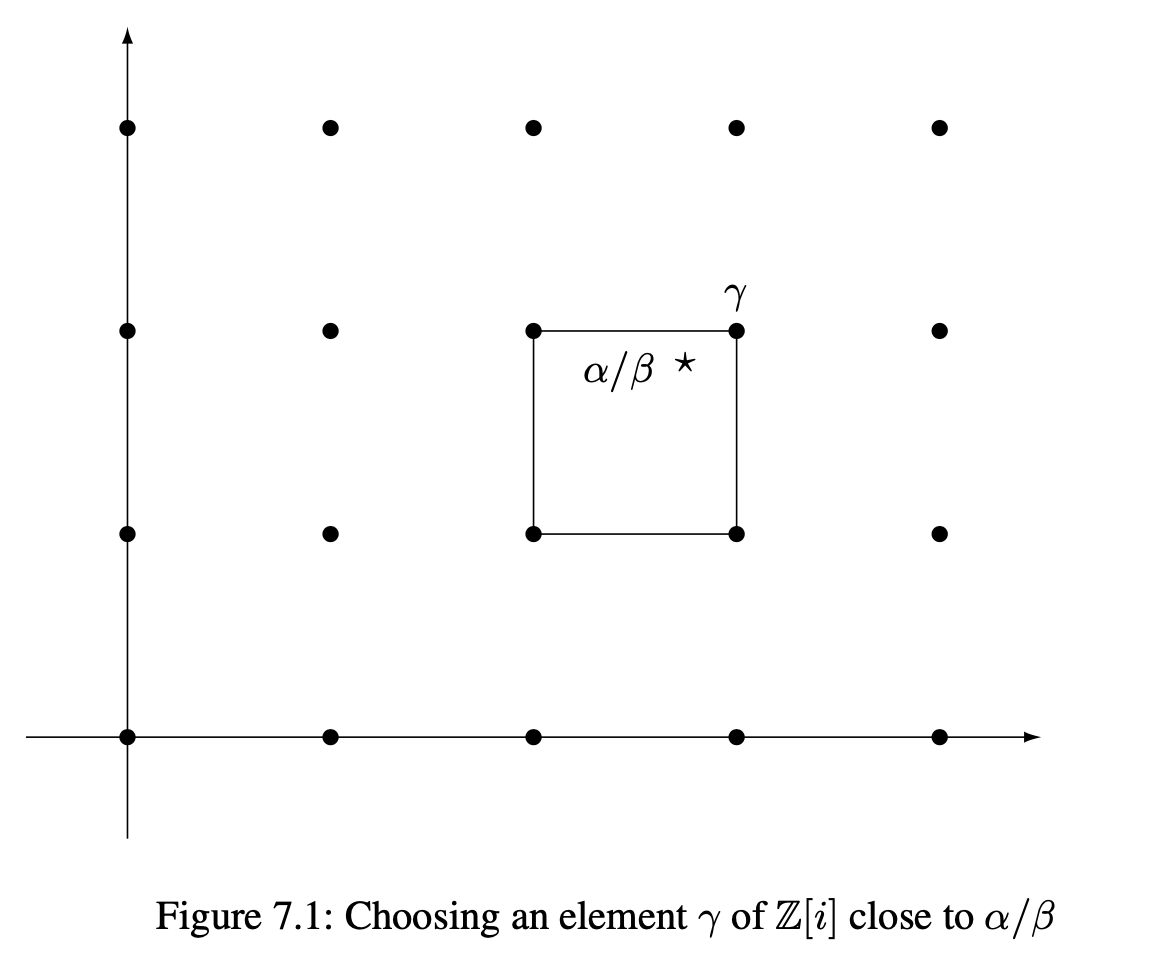
\includegraphics[width=0.5\textwidth]{fig71.png}
  \end{figure}
  Now, we use the fact that regardless of where $\alpha / \beta$ is, its distance to the closest
  corner of the square is at most half of the length of the diagonal of the square; that is, since
  the square's sides have length $1$ and the diagonal thus has length $\sqrt{2}$, we have that for
  any $\alpha,\beta\in \Z[i]$ with $\beta\neq 0$, there exists a $\gamma\in \C$ so that \begin{center}
    Distance from $alpha / \beta$ to $\gamma$ is at most $\frac{\sqrt{2}}{2}$.
  \end{center}
  Since $\sigma(x+yi)=x^2+y^2$ is the square of the distance, we thus have \[
    \sigma\left( \frac{\alpha}{\beta} -\gamma\right) \le \frac{1}{2}
  .\] Multiplying both sides by $\sigma(\beta)$ and using the fact that for any $\zeta_1,\zeta_2\in
  \C$ we have $\sigma(\zeta_1\zeta_2)=\sigma(\zeta_1)\sigma(\zeta_2)$, we get \[
    \sigma(\alpha-\beta\gamma)\le \frac{1}{2}\sigma(\beta)
  .\] Let $\rho=\alpha-\beta\gamma$, so $\alpha=\beta\gamma+\rho$ is automatically true, and we
  further have \[
    \sigma(\rho)\le \frac{1}{2}\sigma(\beta)<\sigma(\beta)
  ,\] since our assumption that $\beta\neq 0$ means $\sigma(\beta)>0$. Thus $\Z[i]$ is a Euclidean
  domain.
\end{proof}

Finally, we explore some useful properties of PIDs.
\begin{theorem}{}
  Let $R$ be a PID, and let $c\in R$ with $c\neq 0$. Then the following are equivalent:
  \begin{enumerate}
    \item $c$ is irreducible.
    \item The principal ideal $cR$ is maximal.
    \item The quotient ring $R/cR$ is a field.
    \item The principal ideal $cR$ is prime.
    \item The quotient ring $R / cR$ is an integral domain.
  \end{enumerate}
\end{theorem}
\begin{proof}[Proof]
  Note that \[
    R /cR~\text{is a field}~\iff cR~\text{maximal}~\implies cR~\text{prime}~\iff R / cR ~\text{is an
    integral domain}
  \] follow directly from Theorem 3.40 and Corollary 3.41. Thus, we only need to prove that $cR$
  prime implies $c$ irreducible, and $c$ irreducible implies $cR$ maximal.

  Suppose that $c$ factors into $ab$. We wish to show that either $a$ or $b$ is a unit. Since
  $ab=c\in cR$, the definition of a prime ideal tells us that either $a\in cR$ or $b\in cR$.
  Without loss of generality, suppose $a\in cR$. Then $a=cr$ for some $r\in R$, so \[
    c=ab=crb
  .\] Since $R$ is an integral domain and $c\neq 0$, we need $rb=1$ (since $c(rb-1)=0$, $c\neq 0$,
  and $R$ integral domain means $rb-1=0$). Hence $b\in R^*$, so $c$ is irreducible.

  Now, suppose $c$ irreducible and let $I\subseteq R$ be an ideal satisfying \[
    cR\subseteq I\subseteq R
  .\] We wish to show that $cR$ is maximal; that is, either $I=cR$ or $I=R$. Since $R$ is a PID, we
  can find some $a\in R$ such that $I=aR$. In particular, \[
    c\in cR\subseteq I=aR
  ,\] so $c=ab$ for some $b\in R$. Since $c$ irreducible, either $a$ or $b$ is a unit:
  \begin{itemize}
    \item If $a$ unit, then $aR=R$, so $I=R$.
    \item If $b$ unit, then $I=aR=c b^{-1}R=cR$.
  \end{itemize}
  Hence $cR$ is a maximal ideal.
\end{proof}

\section{Factorization in Principal Ideal Domains}
Now, we'll prove that every Euclidean domain (and thus PID) is automatically a unique factorization
domain (UFD). From Section 7.2, this will then show that $\Z,\ \Z[i]$, and $F[x]$ are unique
factorization domains. Indeed, even more generally every PID is a UFD (since not all PIDs are
Euclidean domains); make sure to prove this as an exercise!

We start by generalizing the notion of divisibility, then follow with a fundamental divisibility
property in PIDs.
\begin{definition}[Divisibility]{}
  Let $R$ be an integral domain, and let $a,b\in R$ be elements of $R$. We say that $b$
  \textbf{divides} $a$, or $b\mid a$, if there is some element $c\in R$ satisfying $a=bc$. We
  observe that $b\mid a$ is equivalent to the assertion that $a$ is in the ideal $bR$, which in turn
  is equivalent to the inclusion $aR\subseteq bR$.
\end{definition}
\begin{proposition}{}
  Let $R$ be a principal ideal domain, and let $a,b,c\in R$. Suppose that $a$ is irreducible and
  that $a\mid bc$. Then either $a\mid b$ or $a\mid c$, or both.
\end{proposition}
\begin{proof}[Proof]
  Consider the ideal generated by $a$ and $b$, \[
    I=\{ar+bs\mid r,s \in R\} 
  .\] The assumption that $R$ is a PID tells us that $I$ is principal, so \[
    I=dR
  \] for some $d\in R$.

  We know that $a\in I=dR$, so $a=de$ for some $e\in R$. But $a$ is irreducible, so either $d$ or
  $e$ is a unit. This gives us two cases:
  \begin{itemize}
    \item If $e\in R^*$, then $d=e^{-1}a$. But we also know that $b\in I=dR$, so $b=df$ for some
      $f\in R$. Hence $b=e^{-1}af=e^{-1}fa$, so $a\mid b$.
    \item If $d\in R^*$, then $1=dd^{-1}\in dR=I$, so we can find some $r,s \in R$ such satisfying
      \[
        1=ar+bs
      .\] Multiplying both sides by $c$, we get \[
        c= acr+bcs
      .\] Since we assumed $a\mid bc$, we can write $bc=ag$ for some $g\in R$. Substituting and
      factoring yields \[
        c=acr+ags=a(cr+gs)
      ,\] so $a\mid c$.
  \end{itemize}
  Thus if $a\mid bc$ and $a$ irreducible, then either $a\mid b$ or $a\mid c$.
\end{proof}
\begin{corollary}{}
  Let $R$ be a principal ideal domain, and let $a,b_1,\ldots,b_n\in R$. Suppose $a$ is irreducible
  and $a$ divides the product $b_1\cdot \ldots\cdot b_n$. Then there is at least one index $i$ such
  that $a$ divides $b_i$.
\end{corollary}
\begin{proof}[Proof]
  We proceed with induction on $n$. The statement is clearly true for $n=1$, and we just proved the
  case when $n=2$. Assume now that $n\ge 3$ and the statement is true for a product of $n-1$
  factors. We group the $n$ factors as \[
    b_1\cdot \ldots\cdot b_n=\underbrace{b_1}_\text{b}\cdot \underbrace{(b_2\cdot \ldots\cdot
    b_n)}_\text{c}
  .\] Then $a\mid bc$ and $a$ irreducible (given), so the above theorem shows that either $a\mid b$
  or $a\mid c$. The first case is easy, since if $a\mid b$, then we're done (simply set $i=1$). In
  the second case, we're given that $a\mid c$. Since $c$ is the product of $n-1$ factors
  $b_2,\ldots,b_n$, the induction hypothesis tells us that some index $i$ satisfies $a\mid b_i$.
\end{proof}

Before approaching the main theorem of this section, we make an observation about size functions and
units, whose proof is left as an exercise.
\begin{theorem}{}
  Let $R$ be a Euclidean domain with size function $\sigma$, and let $u\in R$. Then $u\in R^*$ if
  and only if $\sigma(u)=1$.
\end{theorem}

\begin{theorem}[PIDs are UFDs]{}
  Let $R$ be a principal ideal domain. Then $R$ is a unique factorization domain.
\end{theorem}
\begin{proof}[Proof]
  We first wish to show that every non-zero non-unit element of $R$ is a product of irreducible
  elements. We're going to make the stronger assumption that $R$ is a Euclidean domain; that is, $R$
  has a size function $\sigma$. [TODO: Prove the more general case for any PID]

  Let's consider the set of counterexamples to our goal: \[
    S=\{~\text{non-zero non-unit}~a\in R\mid a~\text{is \underline{not} a product of irreducibles}\} 
  .\] If $S$ is the empty set, we're done, so assume $S\neq \varnothing$.

  Consider the sizes $\sigma(a)$ of all elements $a\in S$, and choose an element $a'$ of smallest
  size. In other words, we select an $a'\in S$ such that for every $a\in S$, \[
    \sigma(a')\le \sigma(a)
  .\] Since $a'$ is not irreducible (otherwise it wouldn't be in $S$), we can factor $a'=a_1\cdot
  a_2$ such that neither $a_1$ or $a_2$ are units. But then \[
    \sigma(a')=\sigma(a_1)\sigma(a_2)~\text{with}~\sigma(a_1)\ge 2~\text{and}~\sigma(a_2)\ge 2
  ,\] since non-unit elements have size strictly bigger than $1$. It follows that
  $\sigma(a_1)<\sigma(a')$ and $\sigma(a_2)<\sigma(a')$, so neither $a_1$ nor $a_2$ are in $S$
  (since $a'$ is the smallest-sized element in $S$).

  Thus, $a_1$ and $a_2$ are ``not not'' products of irreducibles; that is, they can be represented
  as products of irreducibles. But then $a'=a_1a_2$ is a product of irreducibles, contradicting
  $a'\in S$. Thus $S$ is empty, and so every non-zero non-unit element in $R$ is a product of
  irreducibles. 

  Now, we must show that this factorization into irreducible elements is essentially unique. For
  this, we only assume that $R$ is a PID. Assume that $a\in R$ is written as \[
    a=b_1\cdot \ldots\cdot b_n=c_1\cdot \ldots\cdot c_m
  \] with irreducible elements $b_1,\ldots,b_n,\ c_1,.\ldots,c_m$. In particular, this implies that
  \[
    b_1\mid c_1\cdot \ldots\cdot c_m
  .\] Since $b_1$ is irreducible and $R$ is a PID, by Corollary 7.3.1 (7.16) to deduce that for some
  index $i$, we have $b_1\mid c_i$. Relabeling the other elements, we get $b_1\mid c_1$.

  This means that $c_1=b_1u_1$ for some $u_1\in R$. However, since $c_1$ is also irreducible and
  $ b_1$ is not a unit (since it's irreducible), we see that $u_1$ is a unit.

  Cancelling $b_1$ from both sides (since integral domains have the cancellation property), we
  obtain \[
    b_2\cdot b_3\cdot \ldots\cdot b_n=u_1\cdot c_2\cdot c_3\cdot \ldots\cdot c_m
  .\] We repeat the above argument with $b_2$; note that $b_2$ cannot divide $u_1$ since it's
  irreducible, so after relabeling, we find that $c_2=b_2u_2$ for some unit $u_2$. Canceling $b_2$
  gives \[
    b_3\cdot \ldots\cdot b_n=u_1\cdot u_2\cdot c_3\cdot \ldots\cdot c_m
  .\] Continuing in this fashion, either all of the $b_i$ are gone, or else all of the $c_j$ are
  gone. But then one side is a unit, so the other side cannot have any irreducible elements left. In
  other words, we must have $n=m$, and with step-by-step relabeling, we have $c_i=b_iu_i$ with
  $u_i\in R^*$ for every $i$.

  Thus every PID is a UFD.
\end{proof}

As an easy corollary, we get the following result (since each are PIDs).
\begin{corollary}{}
  $\Z$, $\Z[i]$, and $F[x]$ are unique factorization domains.
\end{corollary}
\begin{example}
  [TODO: Finish proof] As a counterweight to the theorem, it's worthwhile to look at a ring that is
  \textbf{not} a $UFD$. Consider the ring \[
    R=\Z[\sqrt{-3}]=\{a+b\sqrt{-3}\mid a,b\in \Z \} 
  .\] It is a subring of the field of complex numbers. The number $4\in R$ can be factored into \[
  4=2\cdot 2=(1+\sqrt{-3})(1-\sqrt{-3})
  .\] 
\end{example}

\section{The Chinese Remainder Theorem}
The first instance of the Chinese Remainder Theorem appeared over 1500 years ago, in a Chinese
mathematical work by Master Sun: \begin{center}
  We have a number of things, but we do not know exactly how many. If we count them by threes, we
  have two left over. If we count them by fives, we have three left over. If we count them by
  sevens, we have two left over. How many things are there?
\end{center}

We know that a congruence of the form \[
  ax\equiv b\Mod{m}
\] has a solution provided that $\gcd{(a,m)}=1$. The Euclidean algorithm even provides an efficient
way to compute the solution. The simplest version of the Chinese Remainder Theorem (CRT) deals with
the case of two simultaneous linear congruences with different moduli.

\begin{theorem}[Chinese Remainder Theorem, v1]{}
  Let $m_1,m_2\in \Z$ be non-zero integers with $\gcd{(m_1,m_2)}=1$ and let $c_1,c_2\in \Z$.
  \begin{enumerate}
    \item There is a solution $x\in \Z$ to the simultaneous congruences \[
          x\equiv c_1\Mod{m_1}~\text{and}~x\equiv c_2\Mod{m_2}
      .\] 
    \item If $x,x'$ are two solutions, then \[
        x_1\equiv x_2\Mod{m_1m_2}
    .\] 
  \end{enumerate}
\end{theorem}
Before providing a proof, we illustrate the Chinese Remainder Theorem using an example. Suppose we
want to solve \[
  x\equiv 8\Mod{11}~\text{and}~x\equiv 3\Mod{17}
.\] From the first equivalence, we can have $x=8$; but we could also have $x=-3,19,\ldots$. Indeed,
any solution to the first congruence looks like \[
  x=8+11y~\text{for some integer}~y
.\] We explore this flexibility by substituting, \[
  8+11y\equiv 3\Mod{17}\implies 11y\equiv-5\equiv 12\Mod{17}
.\] To solve this, we simply multiply both sides by the inverse of $11$ modulo $17$. We could use
the Euclidean algorithm, or simply trial-and-error, to reveal that $14\cdot 11\equiv 1\Mod{17}$, so
\[
  y\equiv 14\cdot 11y\equiv 14\cdot 12\equiv_168\equiv 15\Mod{17}
.\] So, we have $y=15$, and substituting into $x=8+11y$, we get $x=173$ to solve the simultaneous
congruences.
\begin{proof}[Proof]
  \begin{enumerate}
    \item We start with the first congruence, and observe (like above) that any solution in the form
      \[
        x=c_1+m_1y~\text{for some}~y\in \Z
      \] solves the congruence. Now, we just need to choose a $y$ so that $x$ is also a solution to
      the second congruence $x\equiv c_2\Mod{m_2}$. In other words, we want to find an integer $y$
      that satisfies \[
        c_1+m_1y\equiv c_2\Mod{m_2}
      ,\] or equivalently \[
        m_1y\equiv c_2-c_1\Mod{m_2}
      .\] We know from Theorem 1.39 that this has a solution if and only if $\gcd{(m_1,m_2)}=1$; but
      we know this is true by assumption. Thus, there exists a $y$ so that $x$ solves the
      simultaneous congruences, as desired.
    \item If $x$ and $x'$ are both solutions to the given congruences, we have \[
      x-x'\equiv c_1-c_1\equiv 0\Mod{m_1}~\text{and}~x-x'\equiv c_2-c_2\equiv 0\Mod{m_2}
    .\] Thus $x-x'$ is divisible by both $m_1$ and $m_2$. Since $\gcd{(m_1,m_2)}=1$, we conclude
    that $x-x'$ is divisible by the product $m_1m_2$; in other words, \[
      x\equiv x'\Mod{m_1m_2}
    .\] 
  \end{enumerate}
\end{proof}
\begin{remark}
  Here's a more modern way to state the Chinese Remainder Theorem, using product rings. Consider the
  natural homomorphism \begin{align*}
    \phi: \Z / m_1m_2\Z &\longrightarrow \Z /m_1\Z\times \Z / m_2\Z \\
    a\bmod{m_1m_2} &\longmapsto (a\bmod{m_1},a\bmod{m_2})
  .\end{align*}
  The CRT is equivalent to the assertion that if $\gcd{(m_1,m_2)}=1$, then the map $\phi$ is a ring
  isomorphism. More precisely, CRT(a) says that $\phi$ is surjective (since every simultaneous
  congruence has a solution, so there always exists an $a\in \Z$ that satisfies the requirements),
  and CRT(b) says that $\phi$ is injective (since if two solutions work, then they are congruent).
\end{remark}

There are many ways to generalize the CRT; for example, we could solve a longer list of simultaneous
congruences, work with rings other than $\Z$, etc. Here, we provide a more general version, but
[TODO: include exercise] we can prove a more general result.

\begin{theorem}[Chinese Remainder Theorem, v2]{}
  Let $R$ be a commutative ring, and let $c_1,\ldots,c_n\in R$ be elements having the property
  that\footnote{Note that for $R=\Z$, this property is equivalent to $\gcd{(c_i,c_j)}=1$. Keep this
  in mind when thinking about how this generalizes the CRT.}
  \[
    c_iR+c_jR=R~\text{for all}~i\neq j
  .\] Let $c=c_1c_2\cdots c_n$. Then there is an isomorphism \begin{align*}
    \phi: R /cR &\longrightarrow R /c_1R\times R /c_2R\times \ldots\times R / c_nR \\
    r\bmod{c} &\longmapsto (r\bmod{c_1}, r\bmod{c_2},\ldots,r\bmod{c_n})
  .\end{align*}
\end{theorem}
\begin{proof}[Proof]
  The proof is by induction on $n$. For $n=1$, we have $c=c_1$, and $\phi$ is just the identity map
  $R /cR\to R /cR$. However, in order for the induction step to work, we also need to directly check
  the case of $n=2$ (we will see later why this is the case):
  \begin{lemma}{}
    Let $R$ be an integral domain, and let $a,b\in R$ be non-zero elements satisfying $aR+bR=R$.
    Then there is an isomorphism \[
      \phi:R / abR\longrightarrow R /aR\times R /bR,\ \phi(r\bmod{ab})=(r\bmod{a},r\bmod{b})
    .\] 
  \end{lemma}
  \begin{proof}[Proof]
    We're given that $aR+bR=R$, so we can find elements $u,v\in R$ satisfying \[
      au+bv=1
    \] (since $1\in R$). We start with the map \[
    \psi:R\longrightarrow R/aR\times R/bR,\ \psi(r)=(r\bmod{a}, r\bmod{b})
  .\] We first compute the kernel of $R$. It's clear that $abR\subseteq \ker{(\psi)}$ (since any
  $c\in abR$ is a multiple of both $a$ and $b$, and so is equivalent to $(0,0)$), so we wish to show
  the opposite inclusion $\ker{(\psi)}\subseteq abR$. Let $r\in \ker{(\psi)}$. Then \[
    r\equiv 0\Mod{aR}~\text{and}~r\equiv 0\Mod{bR}
  ,\] so we have \[
    r=as=bt~\text{for some}~s,t\in R
  .\] Multiplying the relation $1=au+bv$ by $s$, we get \[
    s=s(au+bt)=asu+bsv=btu+bsv=b(tu+sv)
  .\] Thus, $b\mid s$, say $s=bw$. Then \[
    r=as=abw\in abR
  .\] Therefore, we get the opposite inclusion $\ker{(\psi)}\subseteq abR$, so equality holds, and
  by Proposition 3.31(c) (the first isomorphism theorem for rings), $\psi$ induces an injective
  homomorphism \[
    \phi:R/abR\hookrightarrow R/aR\times R /bR
  .\] We now only need to verify that $\psi$ is surjective, which shows that $\phi$ is surjective as
  well (and hence an isomorphism). Since $bv=1-au$, we have \[
    \psi(1-au)=\psi(bv)=(1-au\bmod{a}, bv\bmod{b})=(1,0)
  .\] Similarly, we have $au=1-bv$, so \[
    \psi(1-bv)=\psi(au)=(au\bmod{a},1-bv\bmod{b})=(0,1)
  .\] So for any desired $(c,d)\in R /aR\times R /bR$, we have \[
    (c,d)=(c,0)+(0,d)=c(1,0)+d(0,1)=c\psi(bv)+d\psi(au)=\psi(cbv+dau)
  .\] Thus every $(c,d)$ is in the image of $\psi$, and so $\psi$ and $\phi$ are surjective.
  \end{proof}

  We now resume the proof for the CRT. We've shown that it holds for $n=1,2$, so assume that the
  theorem holds for $n$. We then need to prove that it's true for $n+1$.

  Let $c_1,\ldots,c_{n+1}\in R$ as described in the statement (that is, each $c_iR+c_jR=R$ for
  $i\neq j$). In particular, we're given that \[
    c_1R+c_{n+1}R=R=(1),\ \ldots,\ c_nR+c_{n+1}R=1
  .\] Thus, we can find elements in $R$ that satisfy \[
    c_1u_1+c_{n+1}v_1=1,\ldots,c_nu_n+c_{n+1}v_{n}=1
  .\] Multiplying all of these equations together and factoring out $c_{n+1}$, we get \[
    \underbrace{c_1c_2\cdots c_nu_1u_2\cdots u_n}_\text{terms that don't contain
    $c_{n+1}$}+\underbrace{c_{n+1}\cdot (\text{a big mess})}_\text{terms that do contain
  $c_{n+1}$}=1
  .\] This shows that \[
    c_1\cdots c_nR+c_{n+1}R=R
  ,\] which means that we can use the above Lemma with $a=c_1\cdots c_n$ and $b=c_{n+1}$ to deduce
  that there is an isomorphism \[
    R /c_1c_2\cdots c_nR\xrightarrow{\sim}R /c_1c_2\cdots c_nR \times R /c_{n+1}R
  .\] But our induction hypothesis tells us that there's an isomorphism \[
    R /c_1c_2\cdots c_nR\xrightarrow{\sim}R /c_1R\times \ldots\times R /c_nR
  .\] Combining these isomorphisms, we get
  \begin{align*}
    R /c_1c_2\cdots c_nR&\xrightarrow{\sim}R /c_1c_2\cdots c_nR \times R /c_{n+1}R\\
                        &\xrightarrow{\sim}R /c_1R\times \ldots\times R /c_nR\times R /c_{n+1}R
  ,\end{align*} which completes the proof that the theorem holds for $n+1$. Hence by induction, the
  theorem is true for all $n$.
\end{proof}

\subsection{An Application of the Chinese Remainder Theorem}

[TODO]

\section{Field of Fractions}
Now, we wish to show that every integral domain $R$ is a subring of a field, and that there is a
smallest such field $F$. The idea of the proof is to construct $F$ from $R$ just as one constructs
$\Q$ from $\Z$. However, don't be fooled by the assumption that $\Q$ is just the set of fractions
$\frac{a}{b}$; even in $\Q$, we must be careful with the fact that different looking fractions
$\frac{1}{2},\frac{2}{4},\frac{137}{274}$ are really the same quantity.
\begin{theorem}{}
  Let $R$ be an integral domain. There exists a field $F$, called the \textbf{field of fractions of
  $R$}, with the following properties:
  \begin{enumerate}
    \item The ring $R$ is a subring of the field $F$.
    \item If $R$ is also a subring of some other field $K$, then there is a unique injective
      homomorphism $F\hookrightarrow K$ that takes $R$ to itself by the identity map.
  \end{enumerate}
\end{theorem}
\begin{proof}[Proof]
  We must first construct a fraction field $F$ from $R$, in the same way we constructed the field of
  rational numbers $\Q$ from the ring of integers $\Z$, but we must be careful. Let's start with the
  set of pairs \[
    \{(a,b)\mid a,b\in R,\ b\neq 0\} 
  ,\] and we define an equivalence relation $\sim$ on this set by saying that \[
    (a,b)\sim (a',b')~\text{if}~ab'=a'b
  \] (make sure to prove that this is an equivalence relation! This is equivalent to saying that
  $\frac{a}{b}=\frac{a'}{b'}$). We then define $F$ to be the set \[
    F=\{ \text{equivalence classes of pairs $(a,b)$} \}
  .\] We can informally view the pair $(a,b)$ as the fraction $\frac{a}{b}$, but even for $\Q$, the
  fraction $\frac{a}{b}$ is the equivalence class of pairs of integers $(a,b)$ that all correspond to
  the same fraction.

  We want to make $F$ a field, so we need an addition rule and a multiplication rule. We define:
  \begin{align*}
    (a_1,b_1)+(a_2,b_2)&= (a_1b_2+a_2b_1,b_1b_2) \\
    (a_1,b_1)\cdot (a_2,b_2)&=(a_1a_2,b_1b_2)
  .\end{align*}
  Addition may seem weird, but think about how we add $\frac{a_1}{b_1}$ and $\frac{a_2}{b_2}$; these
  are really the same!

  There's a lot to check for well-definedness. First, we need to show that if \[
    (a_1,b_1)\sim (a_1',b_1') ~\text{and}~(a_2,b_2)\sim (a_2',b_2')
  ,\] then the sum $(a_1,b_1)+(a_2,b_2)$ gives the same result as the sum $(a_1',b_1')+(a_2',b_2')$,
  and similarly for their products. 
  [TODO: FINISH DA PROOF]

  Now, we show that this addition and multiplication make $F$ a field. We skip most of the tedious
  proofs of the axioms here, but note that the additive identity is $(0,1)$, and the multiplicative
  identity is $(1,1)$. The additive inverse of any $(a,b)$ will be $(-a,b)$: \[
    (a,b)+(-a,b)=(ab-ab,bb)=(0,bb)\sim (0,1)
  ;\] and for any $(a,b)\not\sim (0,1)$, it has a multiplicative inverse $(b,a)$: \[
    (a,b)\cdot (b,a)=(ab,ab)\sim (1,1)
  .\] We leave the rest for you to check.\\

  Now, we must show that the fraction field $F$ contains a copy of $R$. Consider the map \[
    \phi:R\longrightarrow F,\ a\longmapsto (a,1)
  .\] This is clearly injective, since $(a,1)\sim (b,1)$ if and only if $a=b$. $\phi$ is
  additionally a ring homomorphism, since \[
    \phi(a+b)=(a+b,1)=(a\cdot 1+b\cdot 1,1\cdot 1)=(a,1)+(b,1)=\phi(a)+\phi(b)
  ,\] and \[
  \phi(a\cdot b)=(a\cdot b,1)\sim (a,1)\cdot (b,1)
  .\] Hence $\phi$ is a ring isomorphism from $R$ onto its image (which is in $F$), so $F$ contains a
  copy of $R$.\\

  Finally, we must show that $F$ is the smallest field containing a copy of $R$. What does this mean,
  exactly? If a field $K$ contains $R$, then $K$ also contains $F$; but from above, ``$F$ contains
  $R$'' should be interpreted as saying that there's an injective homomorphism from $R$ to $F$. So,
  we wish to prove: \begin{center}
    If $\phi:R\hookrightarrow F$ and $\psi:R\hookrightarrow K$ are injective ring homomorphisms,
    then there is a unique field homomorphism $\lambda:F\hookrightarrow K$ satisfying $\lambda\circ
    \phi=\psi$.
  \end{center}
  If the map $\lambda$ is going to exist, then for every $a\in R$ we need \[
    \psi(a)=\lambda\circ \phi(a)=\lambda(a,1)
  .\] Therefore, we don't have any choice for the value of $\lambda(a,1)$, since the map $\psi$ is
  already predetermined (from our assumption that $K$ contains a copy of $R$). Next, observe that
  any element $(a,b)\in F$ can be written as \[
    (a,b)=(a,1)\cdot (1,b)=(a,1)\cdot (b,1)^{-1}
  \] (recall that in general, $(a,b)^{-1}=(b,a)$). Since $\lambda$ is required to be a homomorphism,
  we have
  \begin{align*}
    \lambda(a,b)&= \lambda((a,1)\cdot (b,1)^{-1}) \\
                &= \lambda((a,1))\cdot \lambda((b,1))^{-1} \\
                &= \psi(a)\psi(b)^{-1}
  .\end{align*}
  (Since $b\neq 0$ and $\psi$ is injective, $\psi(b)\neq 0$, so $\psi(b)$ has an inverse in the
  field $K$). To reiterate, we've shown that if there is any map $\lambda:F\to K$ satisfying
  $\lambda\circ \phi=\psi$, then it must satisfy \[
    \lambda(a,b)=\psi(a)\psi(b)^{-1}
  .\] We must check that $\lambda$ is well-defined, and is actually a homomorphism. Assume that
  $(a,b)\sim (a',b')$, and inspect $\lambda(a,b)$ and $\lambda(a',b')$. $(a,b)\sim (a',b')$ means
  $ab'=a'b$, so $\psi$ homomorphism means \[
    \psi(a)\psi(b')=\psi(a')\psi(b)
  .\] Hence \[
  \lambda(a,b)=\psi(a)\psi(b)^{-1}=\psi(a')\psi(b')^{-1}=\lambda(a',b')
  ,\] and so $\lambda$ is well-defined.

  [TODO: show $\lambda$ is a homomorphism] Hence $F$ is the smallest field containing $R$.
\end{proof}

Let's look at an important example involving the ring of polynomials $F[x]$. We know that $F[x]$ is
an integral domain, so $F[x]$ has a field of fractions:
\begin{definition}[Field of Rational Functions]{}
  Let $F$ be a field. The \textbf{field of rational functions over $F$} is the fraction field of
  $F[X]$, denoted $F(X)$.
\end{definition}
There's nothing mysterious about $F(X)$; it is simply the field whose elements look like \[
  \frac{\text{polynomial}}{\text{polynomial}},~\text{where the denominator is not the zero
  polynomial}~
,\] with the usual requirement that $\frac{f_1}{g_2}=\frac{f_2}{g_1}$ if $f_1g_2=f_2g_1$. We've
already seen rational functions in calculus, since they're nice to integrate, differentiate, and
graph. However, since we're calling them ``functions'', we must be careful. For instance, given some
$\alpha\in F$, we might try to define the evaluation map \[
  E_\alpha:F(X)\longrightarrow F,\
  E_\alpha(\frac{f(x)}{g(x)})=\frac{E_\alpha(f(x))}{E_\alpha(g(x))}=\frac{f(\alpha)}{g(\alpha)}
.\] However, this isn't always well-defined; what if $g(\alpha)=0$, or both are $0$? [TODO; Exercise
7.17 for a fix]

\section{Multivariate and Symmetric Polynomials}
[TODO: finish]


























\end{document}
